\documentclass[11pt,compress,t,notes=noshow, xcolor=table]{beamer}
\input{../../style/preamble}

% latex-math includes as needed
\input{../../latex-math/basic-math}
\input{../../latex-math/basic-ml}

% Lecture title always has to be there
\title{Algorithms and Data Structures}

\begin{document}

\titlemeta{Matrix Approximation}
{Recommender Systems Application using SVD}
{figure_man/recommender.png}
{
  \item Recommender systems application
}
%\lecture{CIM1 Statistical Computing}

\begin{vbframe}{Application: recommender systems (1)}

\textbf{Initial situation:}
\begin{itemize}
\item $m$ users (e.g. Netflix users)
\item $n$ items (e.g. Movies)
\item $\mathbf{X}$ User-Item Matrix: $x_{ij}$ rating of user $i$ for item $j$
\end{itemize}

\vspace*{0.5cm}

\textbf{Example:} Suppose there are 4 movies and 6 users in our database.

\vspace*{0.5cm}

\begin{footnotesize}
\begin{center}
\begin{table}[h!]
    \centering
    \begin{tabular}{|l|c|c|c|c|}
    \hline
           & \textbf{Die Hard} & \textbf{Top Gun} & \textbf{Titanic} & \textbf{Notting Hill} \\ \hline
    \textbf{User 1} & 5 & \textcolor{red}{NA} & 3 & \textcolor{red}{NA} \\ \hline
    \textbf{User 2} & 5 & 4 & 3 & 3 \\ \hline
    \textbf{User 3} & 2 & \textcolor{red}{NA} & 5 & \textcolor{red}{NA} \\ \hline
    \textbf{User 4} & 5 & 5 & 3 & 1 \\ \hline
    \textbf{User 5} & 1 & 2 & 5 & 5 \\ \hline
    \textbf{User 6} & 1 & 2 & 4 & 5 \\ \hline
    \end{tabular}
  \end{table}    
\end{center}
\end{footnotesize}

Of all available items only a few are evaluated by one user (e.g. Netflix, Amazon), thus the user-item matrix is \textbf{sparse} in many applications.

\lz

\textbf{The target} is to make a \textbf{prediction} for these missing values, which quantifies how high the interest of a user in the respective item is.

\lz

Then we recommend the items that users have not yet rated, but are likely to find interesting.

\framebreak

Basically one distinguishes between two approaches:

\begin{center}
	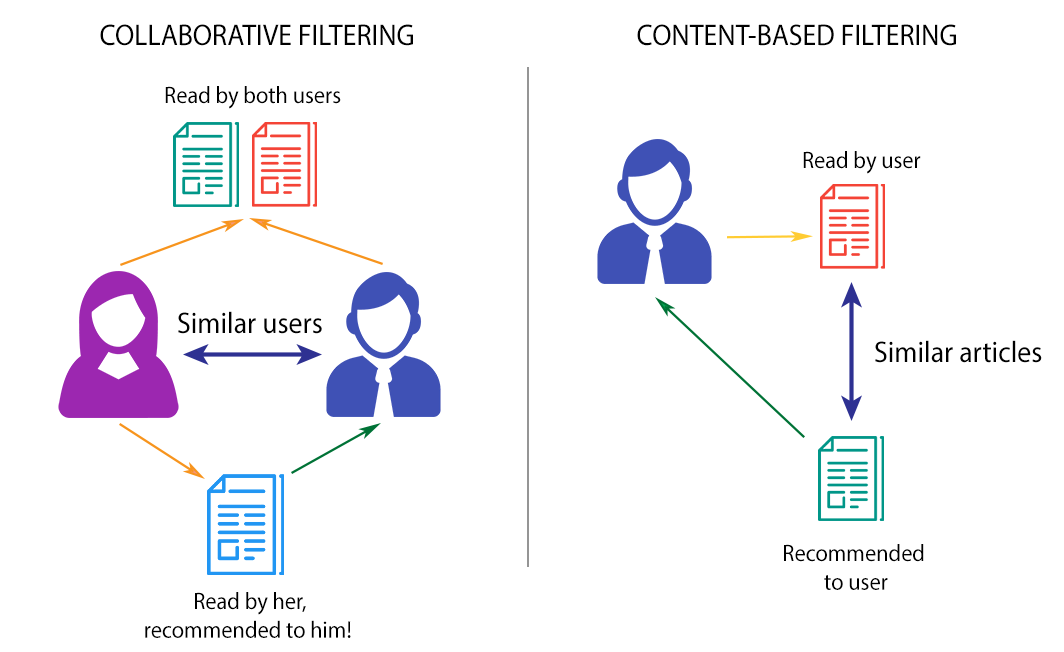
\includegraphics[width = 0.7\textwidth]{figure_man/recommender.png}
\end{center}

\framebreak

\begin{itemize}
\item \textbf{Collaborative Filtering}: Identify "similar" users based on their behavior and recommend items in which similar users are most interested (e.g. by using singular value decomposition).
\item \textbf{Content-based}: Identify - using a similarity measure - "similar" items and recommend items that are similar to the items that the user has rated high in the past.
\end{itemize}

\framebreak

A collaborative filtering approach results from the singular value decomposition.

\textbf{Procedure:}

\begin{enumerate}
\item Fill up the data matrix $\mathbf{X}$ by imputation, e.g.

\begin{itemize}
\item By item average rating, i.e. the column mean value
\item By user average rating, i.e. the row mean value
\item By overall average rating
\end{itemize}
\item Choice of rank $k$: Calculate singular values and select $k$ so that $\sigma_k \gg \sigma_{k + 1}$. Larger $k$ yields a better approximation, smaller $k$ a less complex model.
\item Calculate singular value decomposition of rank $k$ and from it the matrices $\mathbf{W}$ and $\mathbf{H}$.
\item Calculate $\mathbf{W}\mathbf{H}$ and recommend to each user the movies with the best estimated rating from the ones he has not seen yet
\end{enumerate}

\framebreak
Back to the example:
\footnotesize
\begin{verbatim}
X

##         Die Hard   Top Gun   Titanic   Notting Hill
## User 1      5        NA        3           NA
## User 2      5        4         3           3
## User 3      2        NA        5           NA
## User 4      5        5         3           1
## User 5      1        2         5           5
## User 6      1        2         4           5

\end{verbatim}

\normalsize
\begin{enumerate}
\item We replace missing values with the mean value of each row:

\vspace{0.2cm}
\footnotesize
\begin{verbatim}
X = ifelse(is.na(X), rowMeans(X, na.rm = TRUE), unlist(X))
\end{verbatim}


\framebreak
\normalsize
\item Choice of $k$:
\vspace{0.2cm}
\footnotesize
\begin{verbatim}
svd(X)$d
## [1] 17.24 6.13 2.14 0.39
\end{verbatim}

\normalsize
\vspace{0.2cm}
We choose $k = $2.

\item Calculate the matrices $\mathbf{W}$ and $\mathbf{H}$ using a singular value decomposition:
\vspace{0.2cm}
\footnotesize
\begin{verbatim}
res = svd(X, nu = 2, nv = 2)
Uk = res$u
Vk = res$v
Sigmak = diag(res$d[1:2])
W = Uk %*% sqrt(Sigmak)
H = sqrt(Sigmak) %*% t(Vk)
\end{verbatim}


\framebreak
\normalsize
\item Calculate the prediction $\boldsymbol{\hat\mathbf{X}} = \mathbf{WH}$
\footnotesize
\begin{verbatim}
Xhat = W %*% H
\end{verbatim}

%<<echo = F>>=
%options(digits = 2)
%@


%<<echo = F>>=
%X = t(matrix(c(5, NA, 3, NA,
%              5, 4, 3, 3,
%              2, NA, 5, NA,
%              5, 5, 3, 1,
%              1, 2, 5, 5,
%              1, 2, 4, 5), ncol = 6))

%movies = c("Die Hard", "Top Gun", "Titanic", "Notting Hill")
%colnames(X) = movies

%users = c("User 1", "User 2", "User 3", "User 4", "User 5", "User 6")
%rownames(X) = users
%@

%Back to the example:

%<<echo = F>>=
%X = t(matrix(c(5, NA, 3, NA,
%              5, 4, 3, 3,
%              2, NA, 5, NA,
%              5, 5, 3, 1,
%              1, 2, 5, 5,
%              1, 2, 4, 5), ncol = 6))

%movies = c("Die Hard", "Top Gun", "Titanic", "Notting Hill")
%colnames(X) = movies

%users = c("User 1", "User 2", "User 3", "User 4", "User 5", "User 6")
%rownames(X) = users
%@

%<<>>=
%X
%@


%\begin{enumerate}
%\item We replace missing values with the mean value of each row:

%<<>>=
%X = ifelse(is.na(X), rowMeans(X, na.rm = TRUE), unlist(X))
%@

%\item Choice of $k$:

%<<>>=
%svd(X)$d
%@


\begin{footnotesize}
\begin{center}
\begin{table}[h!]
    \centering
    \begin{tabular}{|l|c|c|c|c|}
    \hline
           & \textbf{Die Hard} & \textbf{Top Gun} & \textbf{Titanic} & \textbf{Notting Hill} \\ \hline
    \textbf{User 1} & 4.82 & \textcolor{green}{3.69} & 2.37 & \textcolor{green}{3.41} \\ \hline
    \textbf{User 2} & 5.03 & 3.96 & 2.91 & 3.07 \\ \hline
    \textbf{User 3} & 2.24 & \textcolor{green}{2.70} & 3.64 & \textcolor{green}{5.44} \\ \hline
    \textbf{User 4} & 5.34 & 4.37 & 3.65 & 3.96 \\ \hline
    \textbf{User 5} & 2.87 & 2.90 & 3.85 & 4.52 \\ \hline
    \textbf{User 6} & 1.09 & 1.85 & 4.05 & 5.00 \\ \hline
    \end{tabular}
    \caption{User Ratings for Movies}
  \end{table}    
\end{center}
\end{footnotesize}
\normalsize
Since user 1 is similar to user 2 and user 4 due to their past ratings, we would recommend "Top Gun". However, for user 3 we would recommend "Notting Hill", since this user is more similar to user 5 and user 6 and they rated the movie particularly well.

\end{enumerate}

\framebreak

\textbf{Disadvantages of solution by singular value decomposition:}

\lz

Often the resulting matrices $\mathbf{W}$ and $\mathbf{H}$ are not really interpretable because they contain negative values.

\vspace*{0.2cm}

If the values are naturally non-negative, such as

\begin{itemize}
\item Pixel intensities
\item Counts
\item User scores / ratings
\item ...
\end{itemize}

one often wants to find a non-negative matrix factorization to increase interpretability, i.e. $\mathbf{W}\ge 0$ and $\mathbf{H}\ge 0$ $^{(*)}$.

\vfill

\begin{footnotesize}
 $^{(*)}$ $\ge$ is to be understood component-wise
\end{footnotesize}
\end{vbframe}



\endlecture
\end{document}







